% Desenvolvido por: Prof. Dr. David Buzatto
%
% Versão 1.6.3
% Data: 04/12/2023

\documentclass[
    12pt,
    oneside,
    a4paper,
    chapter=TITLE,
    english,
    french,
    spanish,
    brazil,
]{abntex2}

\usepackage{estrutura}

% ---
% Dados do documento
% ---

\tipotrabalho{Relatório Técnico}

\titulo{Protótipo de um editor de texto inspirado em nano utilizando ncurses em linguagem C}
\subtitulo{NITE: Nano-Inspired Text Editor}

\autor{Fernanda Martins da Silva}
\orientador{Prof. Dr. David Buzatto}

\curso{Bacharelado em Ciência da Computação}
\grau{Bacharel em Ciência da Computação}

\campus{São João da Boa Vista}
\area{TODO: Perguntar ao professor qual a área de concentração do trabalho.}

\local{São João da Boa Vista}
\mes{AGOSTO}
\ano{2025}

\instituicao{%
Instituto Federal de Educação, Ciência e Tecnologia de São Paulo \par Câmpus \imprimircampus }

\preambulo{\imprimirtipotrabalho\ elaborado conforme a ABNT NBR 10719:10, apresentado ao Instituto Federal de Educação, Ciência e Tecnologia
de São Paulo, como parte dos requisitos para a obtenção do grau de \imprimirgrau. \\ \\ Área de Concentração: \imprimirarea}

\setlength{\parindent}{1.3cm}
\setlength{\parskip}{0.2cm}

\makeindex

% ---------------------------------------------------------------------------------
%                                   INÍCIO DO DOCUMENTO
% ---------------------------------------------------------------------------------
\begin{document}
    % Seleciona o idioma do documento
    \selectlanguage{brazil}

    % Retira espaço extra obsoleto entre as frases.
    \frenchspacing

    \pretextual
    \begin{center}
   	
   	\ABNTEXchapterfont\Large\textsc{\imprimirautor}
   	\vspace{2.5cm}
   	
   	\ABNTEXchapterfont\LARGE\textsc{\imprimirtitulo\ifdef{\osubtitulo}{:}{}}

    \ifdef{\osubtitulo}{\ABNTEXchapterfont\Large\imprimirsubtitulo}{}
   	\vspace{2.5cm}
   	   	
   	\hspace{.4\textwidth}
   	\begin{minipage}{.5\textwidth}
   		\SingleSpacing
   		\large\imprimirpreambulo
   		
   		\vspace{\onelineskip}
   		
   		Orientador: \imprimirorientador
   		
        \ifdef{\ocoorientador}{
            \vspace{\onelineskip}
               		
       		Coorientador: \imprimircoorientador
        }{}
        
        
   		
   	\end{minipage}%
    \vfill
   	
   	\Large\textsc{\imprimirlocal}
   	
   	\Large\textsc{\imprimirano}
   	
   	\vspace*{2cm}
   	
\end{center}
    \newcommand{\specialcell}[2][c]{%
	\begin{tabular}[#1]{@{}c@{}}#2\end{tabular}}

\FloatBarrier
\begin{table}[!htbp]
	\centering
	\renewcommand{\arraystretch}{1.5}% Spread rows out...
	\begin{tabular}{| >{\centering}m{2in} | >{\centering}m{2in} | >{\centering\arraybackslash}m{2in} | }
		\hline
		\specialcell[t]{INSTITUTO FEDERAL DE\\EDUCAÇÃO, CIÊNCIA E\\TECNOLOGIA DE SÃO\\PAULO - CÂMPUS SÃO\\JOÃO DA BOA VISTA} & \imprimirmes & \imprimirano \\
		\hline
		\multicolumn{3}{|c|}{\specialcell{
				
				\\ \\
				
				\imprimircurso
				
				\\ \\ \\ \\ \\ \\
				
				\begin{minipage}[t]{0.9\columnwidth}%
				    \centering
				    \ABNTEXchapterfont\LARGE\imprimirtitulo\ifdef{\osubtitulo}{:}{}
                    
                    \ifdef{\osubtitulo}{\ABNTEXchapterfont\Large\imprimirsubtitulo}{}
                    
				\end{minipage}
				
				\\ \\ \\ \\
				
				}}\\
		\multicolumn{3}{|r|}{\specialcell{
				
                \begin{minipage}[t]{0.9\columnwidth}%
   				    \flushright
    				\imprimirautor \ifdef{\ocoorientador}{,}{\ e}
                    \\
                    \imprimirorientador \ifdef{\ocoorientador}{ e\\\imprimircoorientador}{}
                \end{minipage}
				
				\\ \\ \\ \\ \\ \\ \\ \\ \\ \\ 
				
			}}\\
			\hline%                                        todas em letras minúsculas, separadas por ponto e vírgula (;)
		\multicolumn{2}{|l|}{\specialcell{Palavras-chave:\\palavra-chave 1. palavra-chave 2. palavra-chave n.}} & \the\numexpr \getpagerefnumber{LastPage} - 1 \relax \  páginas \\
		\hline
	\end{tabular}
\end{table}
\FloatBarrier

    % ---
    % Inserir a ficha catalográfica
    % ---
    %
% Este é um exemplo de ficha catalográfica.
%
% A ficha catalográfica final deve ser requisitada pelo aluno e inserida neste
% documento para a entrega da versão final.
%

\begin{fichacatalografica}
    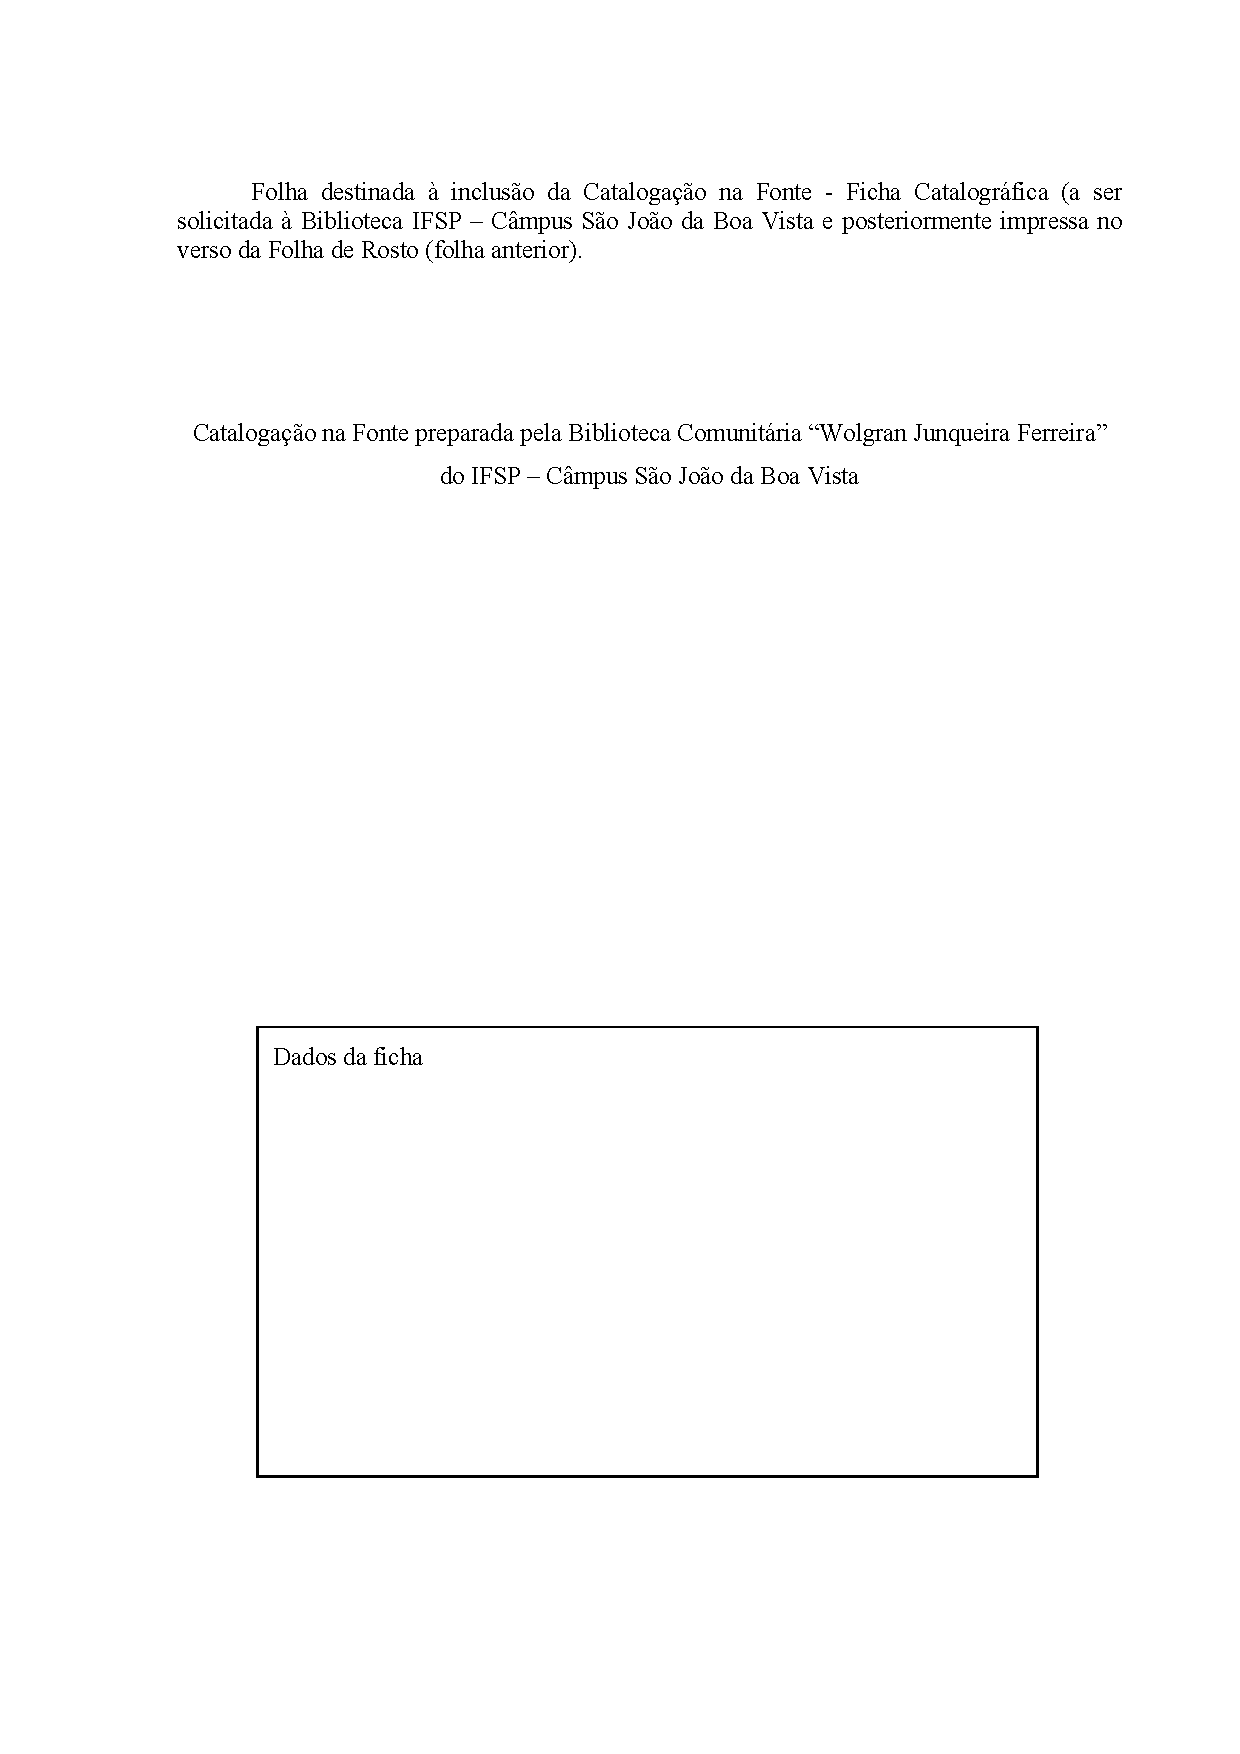
\includepdf{fichaCatalografica/exemploFichaCatalografica.pdf}
\end{fichacatalografica}

    % ---
    % Inserir ata de defesa
    % ---
    %
% Este é um exemplo da ata de defesa.
%
% A ata de defesa será fornecida pelo professor orientador após a defesa do trabalho
% e o orientado será responsável em substituir o arquivo de exemplo pelo arquivo final.
%
\begin{folhadeaprovacao}
	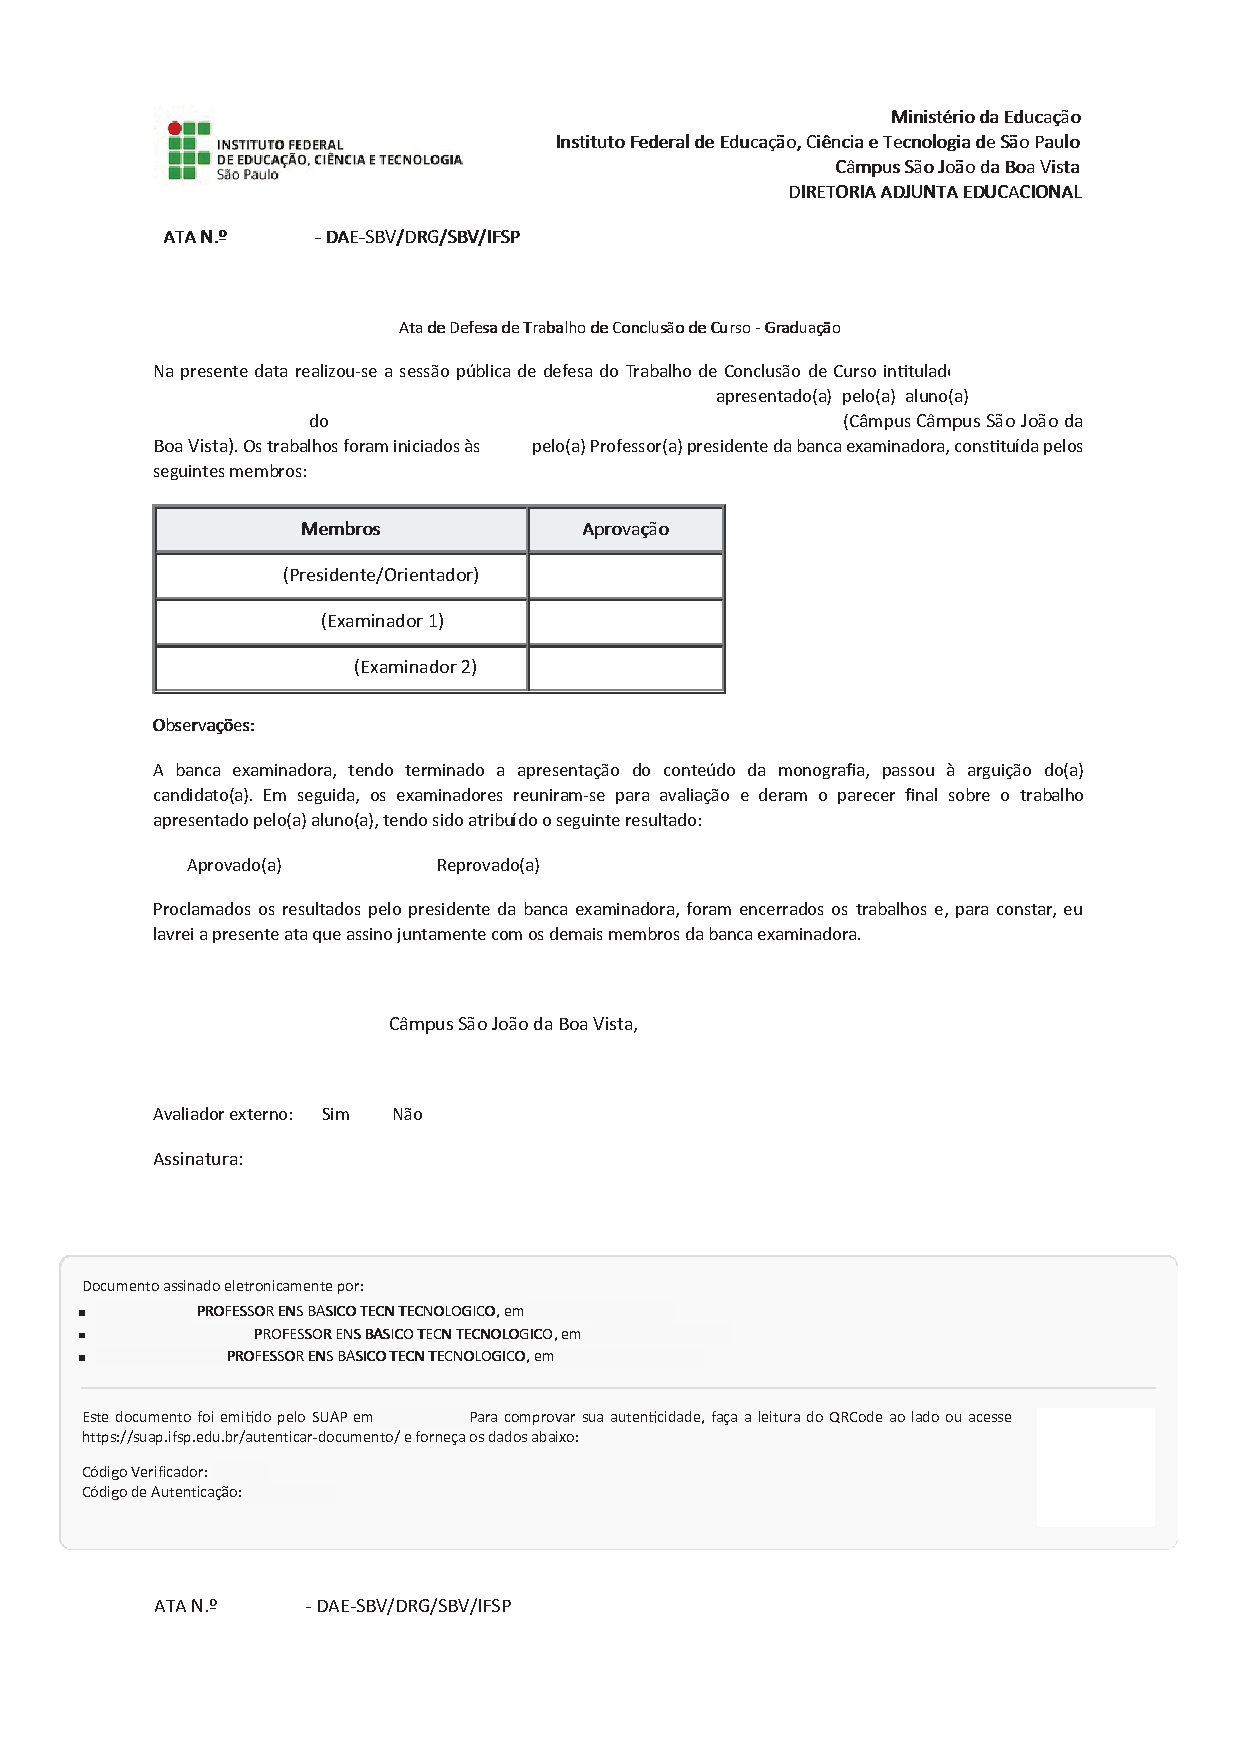
\includepdf[pages={1-}]{ataDefesa/exemploAtaDefesa.pdf}
\end{folhadeaprovacao}

    % ---
    % inserir o sumário
    % ---
    \pdfbookmark[0]{\contentsname}{toc}
    \tableofcontents
    *
    \cleardoublepage
    % ---

    \chapter*{}
\noindent{\textbf{RESUMO}}

\noindent{Neste trabalho é apresentada a formatação que deve ser utilizada nos relatórios técnicos a serem submetidos ao final dos cursos de Graduação e Pós-graduação do IFSP câmpus São João da Boa Vista. Leia com atenção este documento. O máximo de palavras para o resumo é 150 (cento e cinquenta).}

\vspace{\onelineskip}

% todas em letras minúsculas, separadas por ponto e vírgula (;)
\noindent{\textbf{Palavras-chave}: palavra-chave 1. palavra-chave 2. palavra-chave 3. palavra-chave n.}

    \textual
    \chapter{Introdução}
\label{cap:01}

O constante avanço tecnológico impulsiona o desenvolvimento de novas ferramentas e técnicas para atender às demandas da programação.
Diante da diversidade de soluções e editores de texto, os desenvolvedores buscam ferramentas que se adaptem melhor às suas necessidades.
O NITE surge como uma proposta nesse cenário, um editor de linha de comando simples, compacto e poderoso para o desenvolvimento de
aplicações. Inspirado em conceitos modernos e nas funcionalidades de ferramentas predecessoras, busca combinar eficiência e praticidade.
Este trabalho apresenta o estudo de editores e bibliotecas correlatas ao NITE, analisando suas funcionalidades, vantagens e aplicações
práticas, com o objetivo de compreender como elas contribuem para a implementação e evolução de sistemas desse tipo.

\section{Objetivos}

\subsection{Objetivo Geral}

Analisar e compreender as ferramentas e bibliotecas correlatas ao NITE, investigando suas funcionalidades, vantagens e aplicações
práticas no desenvolvimento de sistemas de linha de comando.

\subsection{Objetivos Específicos}
\begin{itemize}
    \item Mapear e descrever ferramentas e bibliotecas relacionadas a edição de texto em terminais, destacando suas principais
    características.
    \item Identificar boas práticas e conceitos modernos aplicados na implementação dessas ferramentas.
    \item Avaliar como essas ferramentas podem contribuir para a evolução e melhoria do NITE.
\end{itemize}

    \chapter{Considerações Gerais}
\label{cap:02}

Texto das considerações gerais, dividido em subseções.

Este é um exemplo de como usar figuras. Referência cruzada: Figura~\ref{fig:exemplo}

\FloatBarrier
\begin{figure}[!htbp]
	\centering
	\caption{Exemplo de figura}
	%scale redimensiona a figura.
	%1.5 = 150% do tamanho original
	%1 = 100% do tamanho original
	%0.20 = 20% do tamanho original
	
\includegraphics[scale=0.4]{imagens/exemploFigura}
	\\\textbf{Fonte:} Elaborada pelo autor
	\label{fig:exemplo}
\end{figure}
\FloatBarrier


Este é um exemplo de como usar tabelas. Referência cruzada: Tabela~\ref{tab:exemplo}

\FloatBarrier
\begin{table}[!htbp]
	\centering
	\caption{Exemplo de tabela de 2 colunas}
	\begin{tabular}{ c | c }
		\hline
		\textbf{Coluna 1} & \textbf{Coluna 2} \\ \hline
		Dado 1a           & Dado 2a           \\ \hline
		Dado 1b           & Dado 2b           \\ \hline
		Dado 1c           & Dado 2c           \\ \hline
		Dado 1d           & Dado 2d           \\ \hline
	\end{tabular}
	\\ \vspace{0.2cm}
	\textbf{Fonte:} Elaborada pelo autor
	\label{tab:exemplo}
\end{table}
\FloatBarrier


Este é um exemplo de como usar quadros. Referência cruzada: Quadro~\ref{qua:exemplo}

\FloatBarrier
\begin{quadro}[!htbp]
	\centering
	\caption{Exemplo de quadro}
	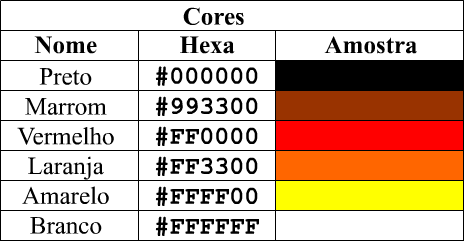
\includegraphics[scale=.7]{imagens/exemploQuadro}
	\\\textbf{Fonte:} Elaborada pelo autor
	\label{qua:exemplo}
\end{quadro}
\FloatBarrier


Este é um exemplo de como usar equações. Referência cruzada: Equação~\ref{eq:exemplo}

\begin{equation}
\sum_{i=1}^{n} i = \frac{n(n+1)}{2}
\label{eq:exemplo}
\end{equation}


Exemplo de inserção de lista de código fonte:

\lstinputlisting[language=Java]{fontes/ClasseExemplo.java} 



Este é um exemplo de como inserir texto sem formatação (ambiente verbatim):

\begin{verbatim}
Texto sem formatação, como espaçamento igual.
\end{verbatim}


Exemplo de lista de itens:

\begin{itemize}
	\item \textbf{Item 1:} texto...;
	\item \textbf{Item 2:} texto...;
	\begin{itemize}
		\item \textbf{Subitem:} texto...;
		\item \textbf{Subitem:} texto...;
		\item \textbf{Subitem:} texto...;
	\end{itemize}
	\item \textbf{Item 3:} texto...;
	\item \textbf{Item n:} texto....
\end{itemize}


Exemplo de lista numerada:

\begin{enumerate}
	\item \textbf{Item:} texto...;
	\item \textbf{Item:} texto...;
	\begin{enumerate}
		\item \textbf{Subitem:} texto...;
		\item \textbf{Subitem:} texto...;
		\item \textbf{Subitem:} texto...;
	\end{enumerate}
	\item \textbf{Item:} texto...;
	\item \textbf{Item:} texto....
\end{enumerate}


Exemplos de comandos para texto e referências:

\begin{itemize}
	\item Para iniciar um novo parágrafo, basta deixar uma linha em branco no código fonte;
	\item Não force o compilador a pular mais de uma linha, pois terá influência negativa na composição do documento;
	\item Sempre deixe o \LaTeX\ realizar a formatação de parágrafos e posicionamento de elementos;
	\item Utilização de aspas simples (abertura \verb|`|, fechamento \verb|'|): `Texto entre aspas simples';
	\item Utilização de aspas duplas (abertura \verb|``|, fechamento \verb|''|): ``Texto entre aspas duplas'';
	\item Negrito (comando \verb|\textbf|): \textbf{texto em negrito};
	\item Itálico (comando \verb|\textit|): \textit{texto em itálico};
	\item Sublinhado (comando \verb|\underline|): \underline{texto sublinhado};
	\item Negrito e itálico (usar comandos juntos): \textbf{\textit{texto em negrito e itálico}};
	\item Alterar cor do texto (comando \verb|\textcolor{cor}{texto}|):
	\begin{itemize}
		\item Exemplo \verb|\textcolor{red}{texto}|: \textcolor{red}{texto vermelho};
		\item Exemplo \verb|\textcolor[RGB]{255, 102, 0}|: \textcolor[RGB]{255, 102, 0}{texto laranja};
		\item Exemplo \verb|\textcolor[HTML]{006AD7}|: \textcolor[HTML]{006AD7}{texto azul};
	\end{itemize}
	\item Ambiente matemático inline (comando \verb|$ expressão $|): $s = x^2-2x +1$;
	\item Referência normal (comando \verb|\cite|):
	\begin{itemize}
		\item \cite{Agaisse1995};
		\item \cite{Abedi2014};
		\item \cite{BtNomenclature2016};
	\end{itemize}
	\item Referência normal com mais de uma obra (comando \verb|\cite|):
	\begin{itemize}
		\item \cite{Abedi2014, Agaisse1995};
        \item \cite{AgapitoTenfen2014, BtNomenclature2016, Nelson2014};
	\end{itemize}
	\item Referência nome e ano (comando \verb|\citeauthorandyear|):
	\begin{itemize}
		\item \citeauthorandyear{Agaisse1995};
		\item \citeauthorandyear{Abedi2014};
		\item \citeauthorandyear{BtNomenclature2016};
	\end{itemize}
\end{itemize}


Exemplo 1 de citação direta:

\begin{citacao}
	Os 20 aminoácidos usualmente encontrados como resíduos em proteínas contém um grupo $\alpha$-carboxil, um grupo $\alpha$-amino e um grupo R distinto substituído no átomo de carbono $\alpha$. O átomo de carbono $\alpha$ de todos os aminoácidos, com exceção da glicina, é assimétrico e, portanto, os aminoácidos podem existir em pelo menos duas formas estereoisoméricas. Somente os estereoisômeros L, com uma configuração relacionada à configuração absoluta da molécula de referência L-gliceraldeído, são encontrados em proteínas \cite[p. 81]{Nelson2014}.
\end{citacao}

Exemplo 2 de citação direta:

\begin{citacao}
	\textit{These various insecticidal proteins are synthesized during the stationary phase and accumulate in the mother cell as a crystal inclusion which can account for up to 25\% of the dry weight of the sporulated cells. The amount of crystal protein produced by a B. thuringiensis culture in laboratory conditions (about 0.5 mg of protein per ml) and the size of the crystals (24) indicate that each cell has to synthesize $10^6$ to $2 \times 10^6$ $\delta$-endotoxin molecules during the stationary phase to form a crystal} \cite[p. 1]{Agaisse1995}.
\end{citacao}

Exemplo de nota de rodapé\footnote{Essa é uma nota de rodapé!}.


\section{Trabalhos Correlatos}

Pesquise e descreva no mínimo três trabalhos correlatos ao seu.

\subsection{Trabalho 1}

Texto...

\subsection{Trabalho 2}

Texto...

\subsection{Trabalho 3}

Texto...
 % TRABALHANDO AQUI
    \chapter{Metodologia}
\label{cap:03}

Idealmente planejado como um projeto incremental, o NITE segue a linha de desenvolvimento
por partes, com implementações lentas e funcionais, como sugere o diagrama abaixo:

\begin{center}
    \begin{tikzpicture}[scale=1.1, transform shape]
        \path[
            mindmap,
            concept color=blue!30,
            text=black,
            level 1/.append style={sibling angle=45, level distance=4.5cm},
            every node/.style={align=center}
        ]
            node[concept, font=\Large\bfseries, minimum size=2.5cm] {NITE}
            [clockwise from=0]
            child[concept color=green!40, grow=0]
            { node[concept, font=\footnotesize, minimum size=2.8cm] {5. Implementar\\atalhos de\\teclado e modos/\\\textit{shortcuts}}}
            child[concept color=orange!40, grow=45]
            { node[concept, font=\footnotesize, minimum size=3.2cm] {4. Implementar\\suporte a\\múltiplos\\arquivos}}
            child[concept color=yellow!70, grow=90]
            { node[concept, font=\footnotesize, minimum size=3.2cm] {3. Implementar\\edição e\\salvamento\\de arquivos} }
            child[concept color=purple!40, grow=135]
            { node[concept, font=\footnotesize, minimum size=3cm] {2. Implementar\\criação e\\abertura de\\arquivos}}
            child[concept color=pink!60, grow=180]
            { node[concept, font=\footnotesize, minimum size=3.2cm] {1. Criar\\protótipo\\inicial e ideia de modos}}
            child[concept color=teal!40, grow=225]
            { node[concept, font=\footnotesize, minimum size=3.5cm] {8. Buscar\\novas\\funcionalidades}}
            child[concept color=red!40, grow=270]
            { node[concept, font=\footnotesize, minimum size=3cm] {7. Implementar\\\textit{syntax}\\\textit{highlight}\footnotemark[1]} }
            child[concept color=lime!60, grow=315]
            { node[concept, font=\footnotesize, minimum size=3cm] {6. Realizar\\ajustes visuais\\e de interface}};
    \end{tikzpicture}
    \footnotetext[1]{Destaque de sintaxe}
\end{center}

Explicando, detalhadamente, cada passo:

\begin{itemize}
    \item \textbf{Primeiro passo:} O primeiro passo consiste na criação de um
        protótipo simples. Idealmente, o protótipo inicial pode se basear na
        interface do Vim e seus derivados, com uma tela de início e atalhos uteis
        a disposição. Além de um protótipo simples, o NITE também será desenvolvido
        com base em dois modos: edição e leitura. Esses modos devem ser analisados
        e implementados posteriormente.

    \item \textbf{Segundo passo:} O segundo passo é a implementação de abrir e
        criar arquivos atravez do NITE, o objetivo aqui é implementar apenas esses
        passos, inicialmente para arquivos de formato *.txt.

    \item \textbf{Terceiro passo:} O tercerceito passo, após a implementação do segundo,
        é garantir que os arquivos possam ser editados e salvos. Aqui, a ideia
        inicial e definida no primeiro passo de dois modos de uso deve ser
        implementado e testado.

    \item \textbf{Quarto passo:} Seguindo, o quarto passo complementa o segundo.
        Aqui deve ser implementado suporte a diversos tipos de arquivos, e de forma
        sucinta abrir e criar esses arquivos.

    \item \textbf{Quinto passo:} O quinto passo tem como objetivo criar e
        implementar atalhos de teclados personalizados para o NITE, baseando em atalhos
        do Vim (e seus derivados), Nano e Emacs (e seus derivados).

    \item \textbf{Sexto passo:} O sexto passo foca em realizar ajustes visuais e
        dar forma ao projeto, trazendo identidade visual. Essa decisão se dá
        pois o foco principal do projeto é funcionalidade, e assim com o tempo aplicar
        caracteristicas visuais unicas.

    \item \textbf{Sétimo passo:} Com o sistema parcialmente pronto, o sétimo passo
        busca implementar destaque de sintaxe para diferentes linguagens de programação.
        Nesta etapa, a biblioteca Tree-Sitter \cite{tree-sitter} será estudada e
        utilizada, gerando árvores de sintaxe abstratas que ajudarão na
        implementação de destaques para diversos tipos de linguagens
        implementadas para o projeto.

    \item \textbf{Oitavo passo:} Por fim, o oitavo passo aponta para futuros estudos
        e avanços do projeto como um todo, onde novas funcionalidades serão
        buscadas e estudadas para versões futuras do NITE.
\end{itemize}

Consequentemente, isso permite testes cuidadosos das funcionalidades
implementadas, além de possibilitar ajustes sempre que necessário de forma ágil e
controlada.

Descrito na sessão anterior, a linguagem de desenvolvimento que mais se adequa a
proposta do projeto foi a linguagem C, por sua confiabilidade e utilização continua
em projetos semelhantes. Nessa lógica a biblioteca utilizada para manipulação de
terminal foi a Ncurses, muito bem fundamentada e completa de funcionaidades que serão
aproveitadas ao máximo. Como ferramentas auxiliares, o uso do Git para versionamento
de arquivos, o editor Zed como IDE principal de desenvolvimento complementar ao
ambiente Linux com o terminal BlackBox para testes. Vale ressaltar aqui o uso do
GCC\footnote{Coleção de compiladores do projeto GNU} como compilador.

Cada etapa do desenvolvimento é realizada em paralelo a análises e estudos do
código-fonte de outros editores, como o NeoVim, com ênfase no código do Nano, editor
que serviu de base para o NITE.
    \chapter{Análise dos Resultados}
\label{cap:04}

Relatar os resultados obtidos a partir dos experimentos e dos estudos realizados. 


\section{Resultados/Impactos}

Resultados.


\section{Orçamento}

Orçamento, caso exista.


\section{Cronograma do Trabalho}

Segue abaixo o cronograma de trabalho das atividades realizadas e das que serão executadas até a Avaliação Final de TCC.

\textbf{Obs:} Para facilitar, crie o cronograma usando o modelo do Word contido no projeto (imagens/templateCronograma.docx), ou qualquer outro \textit{software}, salve a imagem e atualize o arquivo imagens/cronograma.png.

\FloatBarrier
\begin{figure*}[!htbp]
	\centering
	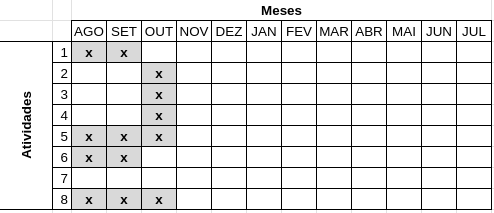
\includegraphics[scale=1]{imagens/cronograma}
\end{figure*}
\FloatBarrier

\begin{enumerate}
	\item Descrição da atividade 1;
	\item Descrição da atividade 2;
	\item Descrição da atividade 3;
	\item Descrição da atividade 4;
	\item Descrição da atividade 5.
\end{enumerate}

    \chapter{Conclusões e Recomendações}
\label{cap:05}

São descritas claramente as conclusões retiradas das discussões e dos experimentos realizados no decorrer da pesquisa,
e finalizada a parte textual do trabalho. Recomendações são declarações concisas de ações, julgadas necessárias a partir das conclusões obtidas,
a serem usadas no futuro. Ou seja, lembre-se de apresentar os possíveis trabalhos futuros derivados do seu trabalho.


    % ----------------------------------------------------------
    % Referências bibliográficas
    % ----------------------------------------------------------
    \postextual
    \bibliography{referencias}
\end{document}
